% -*- latex -*-
%%%%%%%%%%%%%%%%%%%%%%%%%%%%%%%%%%%%%%%%%%%%%%%%%%%%%%%%%%%%%%%%
%%%%
%%%% This TeX file is part of the course
%%%% Introduction to Scientific Programming in C++/Fortran2003
%%%% copyright 2017/8 Victor Eijkhout eijkhout@tacc.utexas.edu
%%%%
%%%% array.tex : basic language elements
%%%%
%%%%%%%%%%%%%%%%%%%%%%%%%%%%%%%%%%%%%%%%%%%%%%%%%%%%%%%%%%%%%%%%

\Level 0 {Introduction}

An \indextermdef{array} is an indexed data structure, that for each
index stores an integer, floating point number, character,
object, et cetera.
In scientific applications, arrays often correspond to vectors and
matrices, potentialy of quite large size. (If you know about the
\acf{FEM}, you know that vectors can have sizes in the millions or beyond.)

In this chapter you will see the C++ \indextermtt{vector} construct,
which implements the notion of an array of things, whether they be
numbers, strings, object.
While C++ can use the C~mechanisms for arrays, for almost all purposes
it is better to use \n{vector}. In particular, this is a safer way to
do dynamic allocation. The old
mechanisms are briefly discussed in section~\ref{sec:staticarray}.

\Level 1 {Initialization}

To define an array you need to declare its size, and you need to give
it its contents. Those actions don't necessarily have to occur
together. (And the contents can later change, as with any other
variable; maybe even the size can change.)
However, 
if you know the array size and contents already before you run your
code, you can create the whole array in one statement. There is more
than one syntax for doing so.
%
\snippetwithoutput{dynamicinit}{array}{dynamicinit}

As you see in this example, if \n{a}~is an array, and \n{i} and
integer, then \n{a[i]} is the i'th element.
\begin{itemize}
\item An array element \n{a[i]} can be used to get the value of an
  array element, or it can occur in the left-hand side of an
  assignment to set the value.
\item The \indextermbus{array}{index} (or
  \indextermbus{array}{subscript}) \n{i} starts numbering at zero.
\item Therefore, if an array has $n$ elements, its last element has
  index~\n{n-1}.
\item If you try to get an array elements outside the bounds of the
  array, the compiler will only detect this in simple cases. More
  likely, your program may give a runtime error, but that does not
  necessarily happen. You could just get some random value.
\end{itemize}

\Level 1 {Ranging over an array}
\label{sec:arrayrange}

If you need to consider all the elements in an array, you typically
use a \n{for} loop. There are various ways of doing this.

First of all consider the cases where you consider the array as a
collection of elements, and the loop functions like a mathematical
`for all'.

\begin{block}{Range over elements}
  \label{sl:array-range}
  You can write a \indextermsub{range-based}{for} loop, which
  considers the elements as a collection.
\begin{verbatim}
for ( float e : array )
  // statement about element with value e
for ( auto e : array )
  // same, with type deduced by compiler
\end{verbatim}

\snippetwithoutput{dynamicmax}{array}{dynamicmax}
\end{block}

(You can spell out the type of the array element, but such type
specifications can be complex. In that case, using \indextermtt{auto} is
quite convenient.)

If you actually need the array index of the element, you can use a
traditional \n{for} loop with loop variable.

\begin{block}{Indexing the elements}
  \label{sl:index-range}
  You can write an \indextermsub{indexed}{for} loop, which uses an
  index variable that ranges from the first to the last element.
\begin{verbatim}
for (int i= /* from first to last index */ )
  // statement about index i
\end{verbatim}
Example: find the maximum element and where it occurs.
%
\snippetwithoutput{idxmax}{array}{idxmax}
\end{block}

\begin{block}{Indexing with pre/post increment}
  \label{sl:prepostindex}
Array indexing in \n{while} loop and such:
\begin{verbatim}
  x = a[i++]; /* is */ x = a[i]; i++;
  y = b[++i]; /* is */ i++; y = b[i];
\end{verbatim}
\end{block}

\begin{exercise}
  \label{ex:array-max}
  Find the element with maximum absolute value in an array. Use:
\begin{verbatim}
vector<int> numbers = {1,-4,2,-6,5};
\end{verbatim}
Which mechanism do you use for traversing the array?

Hint:
\begin{verbatim}
#include <cmath>
..
absx = abs(x);
\end{verbatim}
\end{exercise}

\begin{exercise}
  \label{ex:array-maxidx}
  Find the location of the first negative element in an array.

  Which mechanism do you use?
\end{exercise}

\begin{exercise}
  \label{ex:array-sorted}
  Check whether an array is sorted.
\end{exercise}

\begin{block}{Range over elements by reference}
  \label{sl:array-range-ref}
  Range-based loop indexing makes a copy of the array element. If you
  want to alter the array, use a reference:
  %
  \snippetwithoutput{dynamicscale}{array}{dynamicscale}
\end{block}

\begin{exercise}
  If you do the prime numbers project, you can now do exercise~\ref{sec:arraysieve}.
\end{exercise}

\Level 1 {Vector are a class}
\label{sec:stdvector}

You wouldn't tell it from the above examples, but vectors actually
form a \indextermttdef{vector} class. The angle bracket notation means
that we have a class that is parametrized with the type (see
chapter~\ref{ch:template} for the details), and you can
have vectors of ints, vectors of chars, et cetera. We can now say that
\n{vector<int>} is a type, pronounced `vector-of-int', and you can
make new variables of that type.

What we were doing above was creating an object and initializing it in
one go. Let's decouple these actions.

\begin{block}{Vector definition}
  \label{sl:vector-def}
  Definition, mostly without initialization.
\begin{verbatim}
#include <vector>
using std::vector;

vector<type> name;
vector<type> name(size);
\end{verbatim}
where
\begin{itemize}
\item \n{vector} is a keyword,
\item \n{type} (in angle brackets) is any elementary type or class
  name,
\item \n{name} is up to you, and
\item \n{size} is the (initial size of the array). This is an integer,
  or more precisely, a \n{size_t} parameter.
\end{itemize}
\end{block}

\begin{remark}
  There is also an \indextermttdef{array} class, which at first glance
  looks like a non-resizable variant of \n{vector}. However, it is limited to
  arrays where the size is known at compile time.
\end{remark}

\Level 2 {Vector initialization}

\begin{block}{Vector initialization}
  \label{sl:vector-init}
  You can initialize a vector as a whole:
\begin{verbatim}
vector<int> odd_array{1,3,5,7,9};
vector<int> even_array = {0,2,4,6,8};
\end{verbatim}
(This syntax requires compilation with the \n{-std=c++11}\index{C++11}
option.)
\end{block}

\begin{block}{Vector initialization'}
  \label{sl:vector-initconst}
  There is a syntax for initializing a vector with a constant:
\begin{verbatim}
vector<float> x(25,3.15);
\end{verbatim}
which gives a vector of size~25, with all elements initialized to~3.15.
\end{block}

\Level 2 {Element access}

The simplest way to access vector elements is with the square bracket notation:
\begin{verbatim}
x[1] = 3.14;
cout << x[2];
\end{verbatim}
This gives very fast access, but there is no \emph{checking} on whether the
index is within the \emph{array
  bounds}\index{array!bounds!checking}. Accessing an element outside
the bounds may abort your code, typically with a
\indexterm{segmentation fault}, but your code may just as well
proceed, using invalid data.

There is a safer way to access elements:
\begin{verbatim}
x.at(1) = 3.14;
cout << x.at(2);  
\end{verbatim}
This is slightly slower, but it does perform bounds checking for every access.

\begin{block}{Accessing vector elements}
  \label{sl:vectorsub}
  You have already seen the square bracket notation:
\begin{verbatim}
vector<double> x(5, 0.1 );
x[1] = 3.14;
cout << x[2];
\end{verbatim}
Alteratively:
\begin{verbatim}
x.at(1) = 3.14;
cout << x.at(2);
\end{verbatim}
Safer, slower.
\end{block}

\begin{block}{Ranging over a vector}
  \label{sl:vector-range}
\begin{verbatim}
for ( auto e : my_vector)
  cout << e;
\end{verbatim}
Note that \n{e} is a copy of the vector element:
\snippetwithoutput{vectorrangecopy}{array}{vectorrangecopy}
\end{block}

\begin{block}{Ranging over a vector by reference}
  \label{sl:vector-range-ref}
To set array elements, make \n{e} a reference:
\begin{verbatim}
for ( auto &e : my_vector)
  e = ....
\end{verbatim}
\snippetwithoutput{vectorrangeref}{array}{vectorrangeref}
\end{block}

\begin{exercise}
  \label{ex:range-for}
  Indicate for each of the following vector operations whether you
  prefer to use an indexed loop or a range-based loop.
  \begin{itemize}
  \item Count how many elements of a vector are zero.
  \item Find the location of the last zero.
  \end{itemize}
\end{exercise}

\begin{block}{Vector copy}
  \label{sl:vectorcopy}
  Vectors can be copied just like other datatypes:
  %
  \snippetwithoutput{vectorcopy}{array}{vectorcopy}
\end{block}

\Level 1 {Vector methods}

\begin{exercise}
  \label{ex:vectornormalize}
  Create a \n{vector} $x$ of \n{float} elements, and set them to random
  values.

  Now normalize the vector in $L_2$ norm and check the correctness of
  your calculation, that is,
  \begin{enumerate}
  \item Compute the $L_2$ norm of the vector:
    \[ \| v\| \equiv \sqrt{\sum_iv_i^2} \]
  \item Divide each element by that norm;
  \item The norm of the scaled vector should now by~1. Check this.
  \end{enumerate}
  What type of loop are you using?
\end{exercise}

\begin{slide}{Vector methods}
  \label{sl:vector-method}
  \begin{itemize}
  \item Get elements with \n{ar[3]} (zero-based indexing).\\
    (for C programmers: this is not dereferencing, this uses an
    operator method)
  \item Get elements, including bound checking, with \n{ar.at(3)}.
  \item Size: \n{ar.size()}.
  \item Other functions: \n{front}, \n{back}.
  \item \n{vector} is a `templated class'
  \end{itemize}
\end{slide}

\Level 0 {Vectors are dynamic}
\label{sec:stdvector-dynamic}

There is an important difference between vectors and arrays: a vector
can be grown or shrunk after its creation.
Use the \n{push_back} method to add elements at the end:

\begin{block}{Dynamic extension}
  \label{sl:vector-dynamic}
  Extend with \indextermtt{push_back}:
  %
  \snippetwithoutput{vectorpush}{array}{vectorend}
  %
  also \n{pop_back}, \n{insert}, \n{erase}.\\
  Flexibility comes with a price.
\end{block}

This is not a good way of creating arrays. If you know the size,
create a vector with that size. If the size is not precisely known but
you have a reasonable upper bound, you can 
reserve the vector at that size:
\begin{verbatim}
vector<int> iarray;
iarray.reserve(100);
while ( ... )
  iarray.push_back( ... );
\end{verbatim}

Other methods that change the size: \n{insert}, \n{erase}.

\Level 0 {Vectors and functions}

\Level 1 {Pass vector to function}

\begin{block}{Vector as function argument}
  \label{sl:vector-arg}
  You can pass a vector to a function:
\begin{verbatim}
void print0( vector<double> v ) {
  cout << v[0] << endl;
};
\end{verbatim}
Vectors, like any argument, are passed by value, so the vector is
actually copied into the function.
\end{block}

\begin{block}{Vector pass by value example}
  \label{sl:vector-arg-ex}
  \snippetwithoutput{vectorpassval}{array}{vectorpassnot}  
\end{block}

\begin{exercise}
  \label{ex:vectornormalize-function}
  Revisit exercise~\ref{ex:vectornormalize} and introduce a function
  for computing the $L_2$ norm.
\end{exercise}

\Level 1 {Vector as function return}

\begin{block}{Vector as function return}
  \label{sl:vector-return}
  You can have a vector as return type of a function:
  %
  \snippetwithoutput{vectorreturn}{array}{vectorreturn}
\end{block}

\begin{exercise}
  \label{ex:splitoddeven}
  Write code to take a vector of integers, and construct two
  vectors, one containing all the odd inputs, and one containing all
  the even inputs. So:
\begin{verbatim}
input:
   5,6,2,4,5
output:
   5,5
   6,2,4
\end{verbatim}
\end{exercise}

\begin{exercise}
  \label{ex:splitoddeven-function}
  Revisit exercise~\ref{ex:splitoddeven}. 

  Can you write a function that accepts a vector and returns two
  vectors with the above functionality?
\end{exercise}

\begin{block}{Vector pass by reference}
  \label{sl:vector-arg-ref}
  If you want to alter the vector, you have to pass by reference:
  %
  \snippetwithoutput{vectorpassref}{array}{vectorpassref}  
\end{block}

\begin{exercise}
  \label{ex:vec-rand-sort}
  Write functions \n{random_vector} and \n{sort} to make the following
  main program work:
\begin{verbatim}
int length = 10;
vector<float> values = random_vector(length);
sort(values);
\end{verbatim}
  (This creates a vector of random values of a specified length, and
then sorts it.)

See section~\ref{sec:crand} for the random fuction.
\end{exercise}

\Level 0 {Vectors in classes}

You may want an object that contains a vector, where the size of the
vector is passed to the constructor. Since the class definition is an
abstract definition of all the object, clearly you can not have the
array size there.

\begin{verbatim}
class witharray {
private:
  vector<int> the_array( ???? );
public:
  witharray( int n ) {
    thearray( ???? n ???? );
  }
}
\end{verbatim}

\begin{slide}{Can you make a class around a vector?}
  \label{sl:class-with-vector}
  Vector needs to be created with the object, so you can not have the
  size in the class definition
\begin{verbatim}
class witharray {
private:
  vector<int> the_array( ???? );
public:
  witharray( int n ) {
    thearray( ???? n ???? );
  }
}
\end{verbatim}
\end{slide}

The solution is to specify a vector without size in the class
definition, which creates a vector of size zero. When you create an
object, you then create a vector of the right size, and write that
over the vector member of the object.

\begin{block}{Create and assign}
  \label{sl:class-has-vector}
  The following mechanism works:
\begin{verbatim}
class witharray {
private:
  vector<int> the_array;
public:
  witharray( int n )
    : the_array(vector<int>(n)) {
  };
};
\end{verbatim}
Better than
\begin{verbatim}
  witharray( int n ) {
    the_array = vector<int>(n);
  };
\end{verbatim}
\end{block}

You could read this as
\begin{itemize}
\item \n{vector<int> the_array} declares a int-vector variable, and
\item \n{thearray = vector<int>(n)} assigns an array to it.
\item Second form copy, first form only move.
\end{itemize}
However, 
technically, it actually does the following:
\begin{itemize}
\item The class object initially has a zero-size vector;
\item the expression \n{vector<int>(n)} creates an anonymous vector
  of size~\n{n};
\item which is then assigned to the variable \n{the_array},
\item so now you have an object with a vector of size~\n{n} internally.
\end{itemize}

\Level 1 {Dynamic size of vector}

It is tempting to use \n{push_back} to create a vector dynamically.

\begin{block}{Dynamic size extending}
  \label{sl:vector-extend}
\begin{verbatim}
vector<int> iarray;
\end{verbatim}
creates a vector of size zero. You can then
\begin{verbatim}
iarray.push_back(5);
iarray.push_back(32);
iarray.push_back(4);
\end{verbatim}
\end{block}

However, this dynamic resizing involves memory management, and maybe
operating system functions. This will probably be
inefficient. Therefore you should use such dynamic mechanisms only
when strictly necessary.

\Level 1 {Timing}

Different ways of acessing a vector can have drastically different
timing cost.

\begin{block}{Vector extension}
  \label{sl:vect-extend-code}
  You can push elements into a vector:
  \verbatimsnippet{vectorflex}

  If you allocate the vector statically, you can assign with \n{at}:
  \verbatimsnippet{vectorat}
\end{block}

\begin{block}{Vector extension}
  \label{sl:vect-extend-code2}
  With subscript:
  \verbatimsnippet{vectorsub}

  You can also use \n{new} to allocate (see section~\ref{sec:cnew}):
  \verbatimsnippet{vectornew}
\end{block}

Timings are partly predictable, partly surprising:
\begin{block}{Timing}
  \label{sl:vector-extend-time}
\begin{verbatim}
  Flexible time: 2.445
  Static at time: 1.177
  Static assign time: 0.334
  Static assign time to new: 0.467
\end{verbatim}
\end{block}

The increased time for \n{new} is a mystery.

So do you use \n{at} for safety or \n{[]} for speed? Well, you could
use \n{at} during development of the code, and insert
\begin{verbatim}
#define at(x) operator[](x)
\end{verbatim}
for production.

\Level 0 {Wrapping a vector in an object}

You may want to a create objects that contain a vector, for instance
because you want to add some methods.
%
\verbatimsnippet{printablevector}

Unfortunately this means you may have to recreate some methods:
%
\verbatimsnippet{vectorinheritat}

\Level 0 {Multi-dimensional cases}

\Level 1 {Matrix as vector of vectors}

\begin{block}{Multi-dimensional vectors}
  \label{sl:multi-vector}
  Multi-dimensional is harder with vectors:
\begin{verbatim}
vector<float> row(20);
vector<vector<float>> rows(10,row);
\end{verbatim}
Vector of vectors.
\end{block}

This is not the best implementation of a matrix, for instance because
the elements are not contiguous. However, let's continue with it for a moment.

\begin{block}{Matrix class}
  \label{sl:matrix-class}
  \verbatimsnippet{matrixclassdef}
\end{block}

\begin{block}{Matrix class'}
  \label{sl:matrix-class-cont}
  Better idea:
\begin{verbatim}
  elements = vector<double>(rows*cols);
  ...
  void get(int i,int j) {
    return elements.at(i*cols+j);
  }
\end{verbatim}
(Even more efficient: use cpp macro)
\end{block}

\begin{exercise}
  \label{ex:matrix-methods}
  Add methods such as \n{transpose}, \n{scale} to your matrix class.

  Implement matrix-matrix multiplication.
\end{exercise}

\Level 1 {A better matrix class}

You can make a `pretend' matrix by storing a long enough \n{vector} in
an object:
%
\verbatimsnippet{matrixclass}

The most important advantage of this is that it is compatible with how
many libraries and codes store a matrix traditionally.

The syntax for \n{set} and \n{get} can be improved.
\begin{exercise}
  Write a method \n{element} of type \n{double&}, so that you can write
\begin{verbatim}
A.element(2,3) = 7.24;
\end{verbatim}
\end{exercise}

\Level 0 {Static arrays}
\label{sec:staticarray}

For small arrays you can use a different syntax. 

\snippetwithoutput{arrayinit}{array}{staticinit}

This has the
(minimal) advantage of not having the overhead of a class
mechanism. On the other hand, it has a number of disadvantages:
\begin{itemize}
\item You can not query the size of an array by its name: you have to
  store that information separately in a variable.
\item Passing such an array to a function is really passing the
  address of its first element, so it is always (sort of) by
  reference.
\end{itemize}

Range-based indexing works the same as with vectors:
%
\snippetwithoutput{rangemax}{array}{rangemax}

\Level 0 {Advanced topics}

\Level 1 {Iterators}
\label{sec:iterator}

You have seen how you can iterate over a vector
\begin{itemize}
\item by a for loop over the indices, and
\item with a range-based loop over the indices.
\end{itemize}
There is a third way, which is actually the basic mechanism underlying
the range-based looping.

An \indextermdef{iterator} is a pointer to a vector element. Mirroring
the index-loop convention of
\begin{verbatim}
for (int i=0; i<hi; i++)
  element = vec.at(i);
\end{verbatim}
you can iterate:
\begin{verbatim}
for (auto elt_ptr=vec.begin(); elt_ptr<vec.end(); ++elt_ptr)
  element = *elt_ptr;
\end{verbatim}
Some remarks:
\begin{itemize}
\item This is one of the very few places where you need the asterisk in C++
  for \indexterm{dereferencing}; section~\ref{sec:cderef}.
\item As with a normal loop, the \n{end} iterator point just beyond the end
  of the vector.
\item You can do \indextermbus{pointer}{arithmetic} on iterators, as
  you can see in the \verb-++elt_ptr- update part of the loop header.
\end{itemize}
Another illustration of pointer arithmetic on iterators is getting the
last element of a vector:
%
\snippetwithoutput{vectorpush}{array}{vectorend}
\snippetwithoutput{vectorpushiterator}{array}{vectorenditerator}

\Level 1 {Old-style arrays}

Static arrays are really an abuse of the equivalence of arrays and
addresses of the C programming language. This appears for instance in
parameter passing mechanisms.

\Level 2 {C-style arrays and subprograms}

Arrays can be passed to a subprogram, but the bound is unknown there.
%
\verbatimsnippet{arraypass}
%
\begin{exercise}
  Rewrite the above exercises where the sorting tester or the maximum
  finder is in a subprogram.
\end{exercise}

Unlike with scalar arguments, array arguments can be altered by a
subprogram: it is as if the array is always passed by reference. This is
not strictly true: what happens is that the address of the first
element of the array is passed. Thus we are really dealing with pass
by value, but it is the array address that is passed rather than its value.

\Level 2 {Multi-dimensional arrays}

Multi-dimensional arrays can be declared and used with a simple extension of
the prior syntax:
\begin{verbatim}
float matrix[15][25];

for (int i=0; i<15; i++)
  for (int j=0; j<25; j++)
    // something with matrix[i][j]
\end{verbatim}

Passing a multi-dimensional array to a function, only the first
dimension can be left unspecified:
%
\verbatimsnippet{arraypass2d}

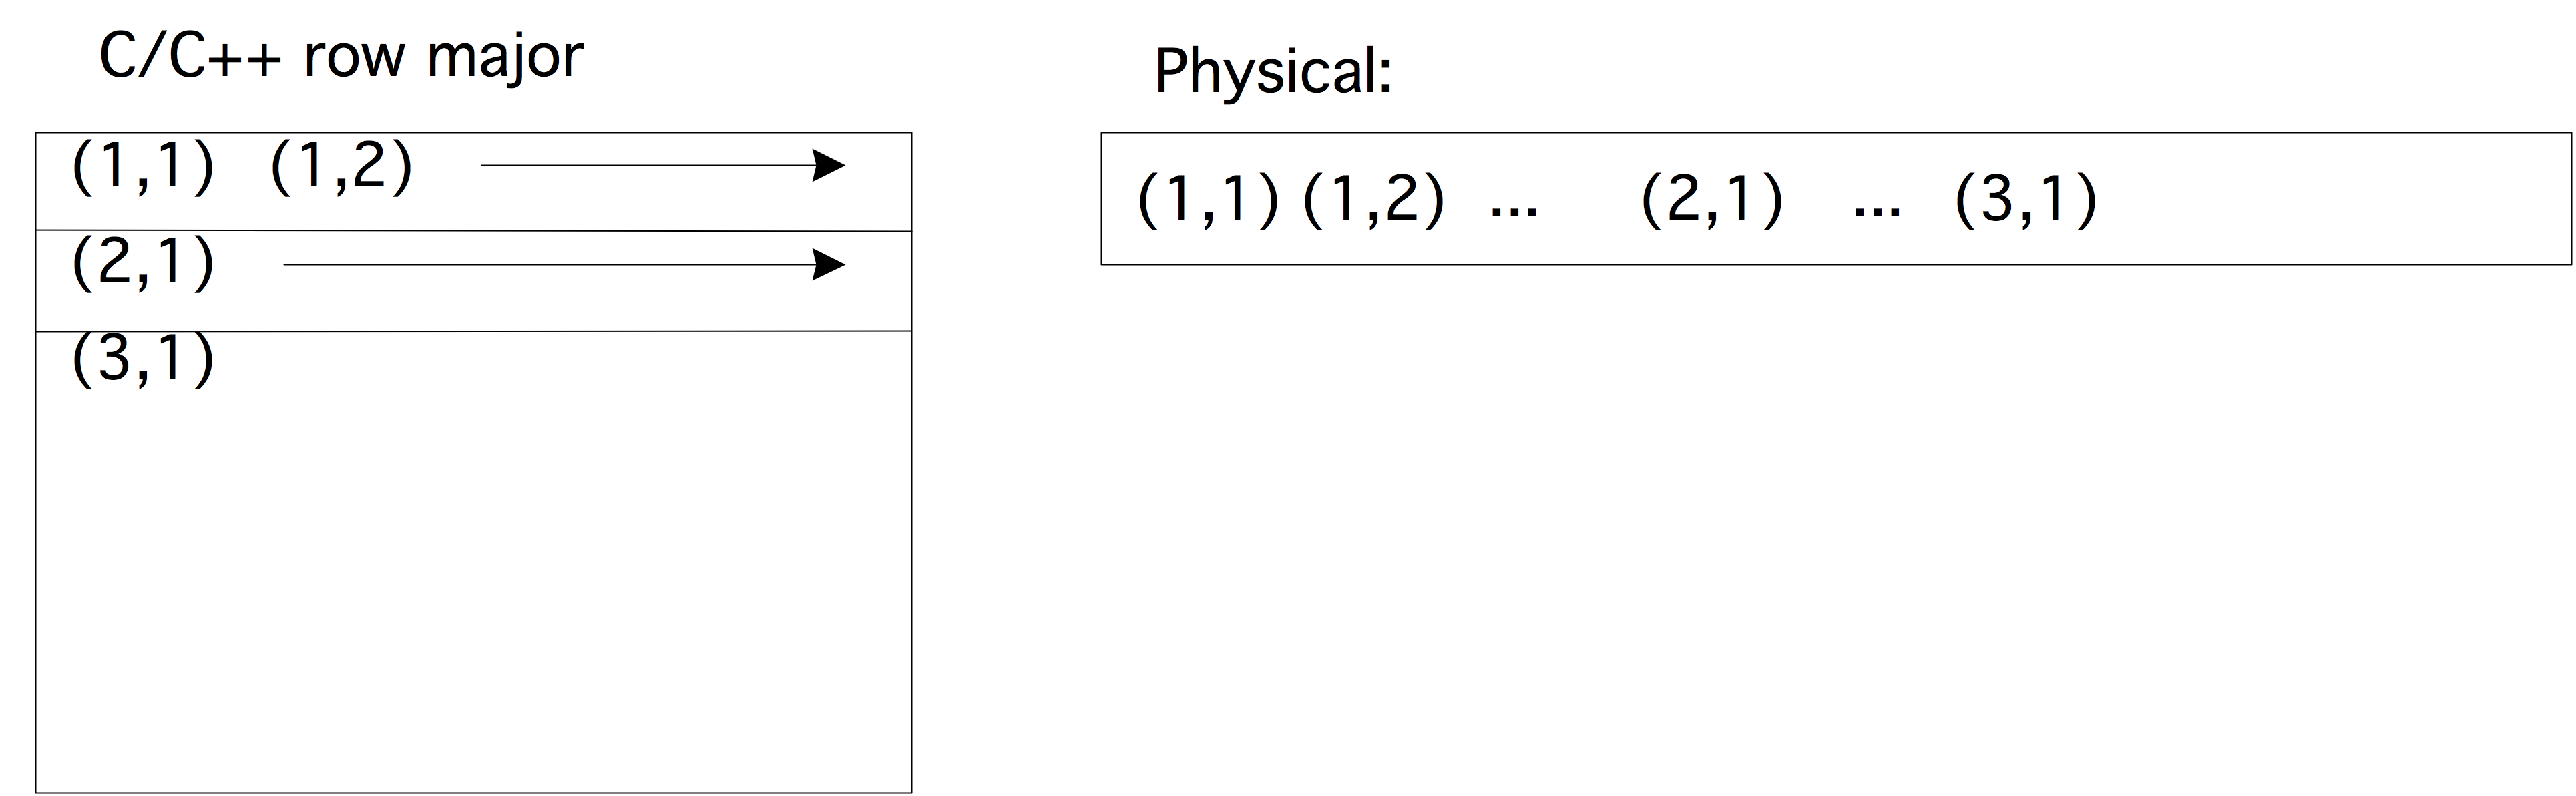
\includegraphics[scale=.1]{arrayc}

\Level 2 {Memory layout}

Puzzling aspects of arrays, such as which dimensions need to be
specified and which not in a function call, can be understood by
considering how arrays are stored in memory.
The question then is how a two-dimensional (or higher dimensional)
array is mapped to memory, which is linear.
\begin{itemize}
\item A one-dimensional array is stored in contiguous memory.
\item A two-dimensional array is also stored contiguously, with first
  the first row, then the second, et cetera.
\item Higher dimensional arrays continue this notion, with contiguous
  blocks of the highest so many dimensions.
\end{itemize}

As a result of this, indexing beyond the end of a row, brings you to the
start of the next row:
%
\verbatimsnippet{arraywrap}

We can now also understand how arrays are passed to functions:
\begin{itemize}
\item The only information passed to a function is the address of the
  first element of the array;
\item In order to be able to find location of the second row (and
  third, et cetera), the subprogram needs to know the length of each
  row.
\item In the higher dimensional case, the subprogram needs to know the
  size of all dimensions except for the first one.
\end{itemize}

\Level 0 {Exercises}

\begin{exercise}
  Program \indexterm{bubble sort}: go through the array comparing
  successive pairs of elements, and swapping them if the second is
  smaller than the first. After you have gone through the array, the
  largest element is in the last location. Go through the array again,
  swapping elements, which puts the second largest element in the
  one-before-last location. Et cetera.
\end{exercise}

\begin{block}{Pascal's triangle}
  \label{sl:pascal-def}
  \small
  Pascal's triangle contains binomial coefficients:
\begin{verbatim}
Row    1:                     1
Row    2:                   1   1
Row    3:                 1   2   1
Row    4:               1   3   3   1
Row    5:             1   4   6   4   1
Row    6:           1   5  10  10   5   1
Row    7:         1   6  15  20  15   6   1
Row    8:       1   7  21  35  35  21   7   1
Row    9:     1   8  28  56  70  56  28   8   1
Row   10:   1   9  36  84 126 126  84  36   9   1
\end{verbatim}
where \[ p_{rc} = \begin{pmatrix} r\\c \end{pmatrix} = \frac{r!}{c!(r-c)! }. \]
The coefficients can easily be computed from the recurrence
\[ p_{rc} = 
\begin{cases}
  1&c\equiv 1\vee c\equiv r\\
  p_{r-1,c-1}+p_{r-1,c}
\end{cases}
\]
\end{block}

\begin{exercise}
  \label{ex:pascal-ex}
  \small
  \begin{itemize}
  \item 
    Write a class \n{pascal} so that \n{pascal(n)} is the object
    containing $n$~rows of the above coefficients. Write a method
    \n{get(i,j)} that returns the $(i,j)$ coefficient.
  \item
    Write a method \n{print} that prints the above display.
  \item
    Write a method \n{print(int m)} that prints a star if the
    coefficient modulo~$m$ is nonzero, and a space otherwise.
\begin{verbatim}
          *
         * *
        *   *
       * * * *
      *       *
     * *     * *
    *   *   *   *
   * * * * * * * *
  *               *
 * *             * *
\end{verbatim}
  \item
    The object needs to have an array internally. The easiest solution
    is to make an array of size $n\times n$.

    Bonus: when you have that code working, optimize your code to use
    precisely enough space for the coefficients.
  \end{itemize}
\end{exercise}

\begin{exercise}
  A knight on the chess board moves by going two steps horizontally or
  vertically, and one step either way in the orthogonal
  direction. Given a starting position, find a sequence of moves that
  brings a knight back to its starting position. Are there starting
  positions for which such a cycle doesn't exist?
\end{exercise}

\begin{exercise}
  Put eight queens on a chessboard so that none threatens any other.
\end{exercise}

\begin{exercise}
  From the `Keeping it REAL' book, exercise 3.6 about Markov chains.
\end{exercise}
